\documentclass[10pt,UTF8]{article}
\usepackage{ctex}
\usepackage{amssymb,amsmath,titlesec}
\usepackage[round]{natbib}
\usepackage[hmargin = 1in, vmargin = 1in]{geometry}
\renewcommand{\refname}{References}
\usepackage[parfill]{parskip}
\usepackage{graphicx}
\usepackage[font=bf]{caption}
\usepackage{titlesec}
\usepackage{booktabs}
\usepackage{multicol}
\usepackage{enumitem}
\usepackage{hyperref}

\newenvironment{Figure}
  {\par\medskip\noindent\minipage{\linewidth}}
  {\endminipage\par\medskip}

%\setlength{\bibsep}{3pt}
%\pagenumbering{\gobble}
%\setlength{\hyphenpenalty}{1000}
%\setlength{\exhyphenpenalty}{1000}

\title{Defeat Most Human: 现代规则的俄罗斯方块游戏AI}
\author{陈益漳\ 成昂\ 黄程宇\ 傅欣毅}
\date{Jan 10th, 2020}


\begin{document}
\maketitle
\section*{摘要}

我们使用Approximate Q-Learning算法训练AI挑战基于现代规则的俄罗斯方块,以击败大多数的人类玩家作为目的。将玩家(AI)可以获取到的所有关于游戏环境的信息,包括以二维数组表示的当前的游戏区域、当前的连击数量、分数、正在下落的方块、hold的方块、未来的方块等信息视为State,将游戏发出的方块放稳在游戏区域的某个位置这一操作视为Action。同时我我们使用线性权重方程和四阶多项式权重方程作为评估函数,并比较两者表现。我们通过随机发送垃圾块来模拟对战,在经过大量的训练后,我们的AI已经可以坚持极长的时间。我们接下来预计让我们的AI能预测更多的方块,能够有计划得做出更复杂的攻击行为。


\begin{multicols}{2}

\section{俄罗斯方块的历史}

俄罗斯方块是世界上最著名的电子游戏之一,有着长达35年的历史。时至今日,在加入了以对战为重点的现代版规则后,俄罗斯方块仍然有许多爱好者。\\
作为一款久负盛名的游戏,俄罗斯方块一直是计算机科学家们研究的对象。现在,传统俄罗斯方块已经有了许多用AI来游玩的解决方案,而我们则想要用AI挑战基于现代规则的俄罗斯方块。\\
在现代规则下,玩家不仅需要努力消块来确保自己不死,还需要争取通过t-spin、四消等方式给对手发送垃圾块,以此来攻击对手,以期获得最终的胜利。\\
任天堂开发的基于现代规则的游戏《Tetris99》,在这个游戏中99个玩家将同时游玩基于现代规则的俄罗斯方块,在保证自己不失败的前提下互相攻击,并最终决出一个胜者。由于不同的基于现代规则的俄罗斯方块游戏在一些细微的规则上都可能会有一定的区别,我们对现代规则的讨论将基于《Tetris99》的规则,以避免产生歧义。
\begin{Figure}
    \centering
    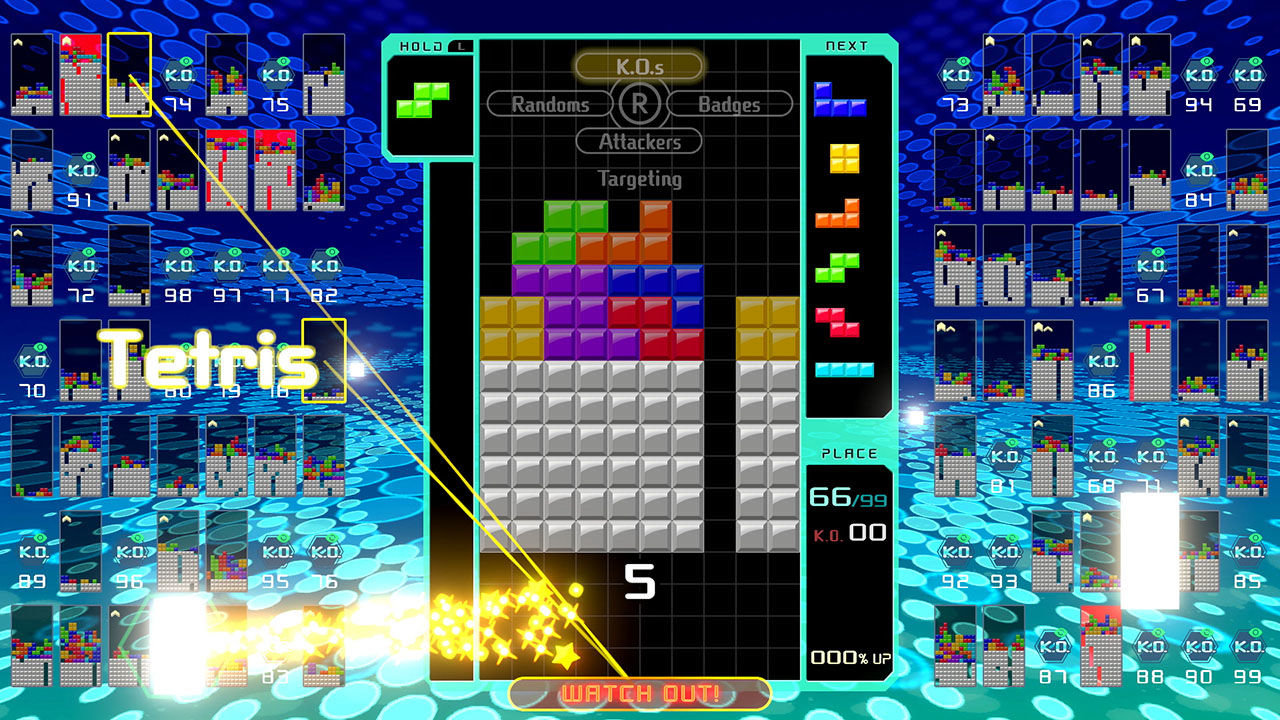
\includegraphics[width=1\textwidth]{figure/Tetris99.png}
    \captionof{figure}{Tetris99}
\end{Figure}

\section{游戏规则}

俄罗斯方块的基本规则是移动、旋转和摆放游戏自动输出的各种方块(S, Z, J, L, T, O, I),使之排列成完整的一行或多行从而消除。游戏失败的条件是方块堆积地过高以至于覆盖住了某一片区域(往往是方块的出生位置)。游戏的基本宗旨是通过积极的消行来避免游戏失败,并且在此基础上发展出了经典规则下的计分玩法以及现代规则下的对战玩法等玩法。

\subsection{游戏目标}
在传统规则的俄罗斯方块下,玩家的游戏目标是在保持游戏不失败的前提下获得较高的分数。游戏的得分方式基本上是通过消行,而消行所得的分数与一次性消除的行数是呈指数关系的,既一次性消行数每增加1,此次消行的得分将乘以2,因此在相同的消行总数下,进行的消四操作越多总分越高。传统俄罗斯方块会随着玩家消行总数的增长增加方块的下落速度,所以为了能够在游戏难度较低的时候获得尽量多的分数,玩家往往会倾向于只使用消四来进行消行,同时使游戏场地中的方块排列尽量规整、高度尽量低。

\begin{Figure}
    \centering
    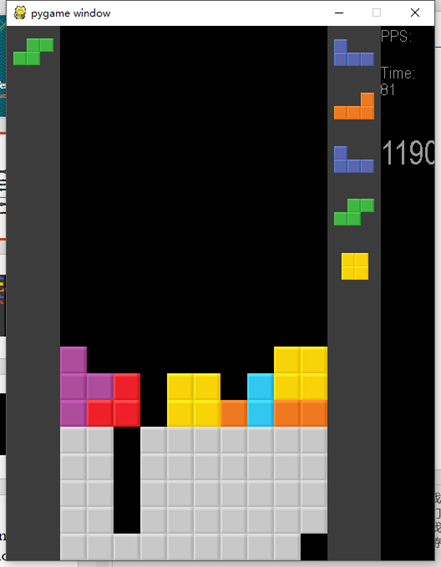
\includegraphics[width=0.5\textwidth]{figure/ours.png}
    \captionof{figure}{我们训练的AI,图中下方的灰色方块就是垃圾快。垃圾块一般一次发送1、2、4、6、8行,从画面底端瞬间出现,呈现为中间空出一列的灰色方块。图中的玩家先接受了一组4行的垃圾块,后接受了一组1行的垃圾块。}
\end{Figure}

但是,当现代规则的俄罗斯方块引入多人游戏模式,并且让玩家能够通过自己的某些特殊操作给对手发送垃圾块后,玩家的目标就成为了在多人对战中存活,或者说,在保证自己不失败的前提下尽量多的对对手进行攻击(即向对手发送垃圾块)。并且,由于现代规则中攻击对手的收益较高,导致很多玩家会将攻击和打击敌人作为自己策略的重点,即使这样会使他们本身变得更容易受攻击而失败。


\subsection{操作}

经典俄罗斯方块中玩家可以进行以下操作:左移,右移,左转,右转,加速下落;而在现代规则的俄罗斯方块中,玩家除了可以进行经典俄罗斯方块中的操作外,还可以进行硬降、hold等操作。

\begin{itemize}
    \itemsep-5pt
    \item 左移与右移:使当前方块左移或右移一格。
    \item 左转与右转:使当前方块逆时针或顺时针旋转。
    \item 加速下落:使当前方块的下落速度增加。
    \item 硬降(Hard Drop):使当前方块瞬间降落。
    \item Hold:如果当前hold槽中有方块,则用槽中的方块和当前方块互换;否则,将当前方块存入hold槽,将下一个方块变为当前方块。
\end{itemize}

\subsection{SRS}

SRS的全称是Super Rotation System,是现代版俄罗斯方块中广泛使用的新的旋转系统。它详细
地定义了各个方块的出生位置以及旋转方式,尤其是“踢墙”的旋转方式。

\begin{Figure}
    \centering
    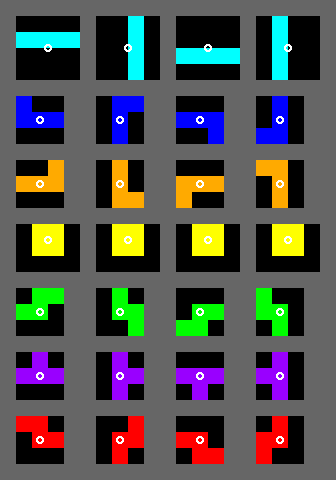
\includegraphics[width=0.5\textwidth]{figure/SRS.png}
    \captionof{figure}{各个方块的中心点以及旋转方式}
\end{Figure}


\subsubsection{关于踢墙(Wall Kick)}

踢墙是SRS和经典俄罗斯方块中的旋转方式的最重要的区别,而由其衍生出的T-Spin等特殊操作更是现代规则中的对战息息相关。踢墙指的是当玩家尝试旋转一个方块,但是方块旋转后的位置和已有的方块重合的情况。在经典规则下,这种旋转被认为是非法的,因此不会产生作用;而在SRS规则下,SRS系统则会对旋转后的方块的周围的位置进行判定,并将方块移动到可能的位置;如果没有合适的位置,则将与经典俄罗斯方块一样,无法旋转。

\begin{Figure}
    \centering
    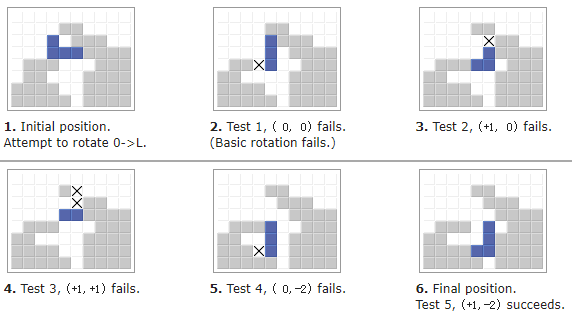
\includegraphics[width=1\textwidth]{figure/kick.png}
    \captionof{figure}{在SRS规则下,一块“J”块想要在图1的情况下进行一次逆时针旋转,但是如图2所示,它旋转后的位置和已有的方块重合了。最后,在经过图3、4、5的尝试后,它终于成功被放在了图6所示的位置中。这一系列的过程在玩家看来都是瞬间完成的,也就是说玩家在图1的状态下进行逆时针操作后,方块瞬间变成了图6所示的位置。}
\end{Figure}

\subsubsection{关于*-Spin}

进行一次*-Spin,指的是用*块(除了O块,因为O块无法踢墙)在SRS规则下进行了一次踢墙操作后成功消行。由于一次*-Spin需要同时满足踢墙操作和消行,因此比较难以实现;不过,如果玩家能在对战中完成一次*-Spin,也将得到相应的收益,比如给对手发送垃圾块等。由于T块最容易被用于构建这种Spin,因此对战中T-Spin最为常用,也是玩家最常见的攻击手段之一。

\begin{Figure}
    \centering
    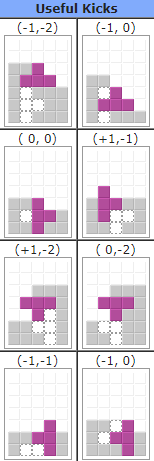
\includegraphics[width=0.3\textwidth]{figure/spin1.png}
    \captionof{figure}{图中展示了一些对战中常用的T-Spin。游戏中,玩家常常会用这些T-Spin对对手进行攻击。}
\end{Figure}

\begin{Figure}
    \centering
    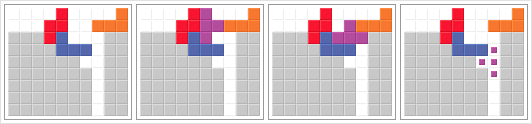
\includegraphics[width=1\textwidth]{figure/spin2.png}
    \captionof{figure}{图中展示了一次T-Spin-Tripple操作——玩家用一次T-Spin操作成功地消除了三行。这种一次消除3行的T-Spin由于需要几个方块的规划和准备以及较强的对局势的预判和观察能力,在对战中较为罕见,也是最强的攻击方式之一,可以一次性给对手发送6行垃圾块。}
\end{Figure}

\subsubsection{攻击}

现代规则给玩家提供了各种攻击对手的方式,比如多消、各种Spin、连击、全消等。为了简化我们的模型,我们只在游戏中实现了了多消、T-Spin、连击这三种攻击方式。\\

以下是它们在实际游戏中的攻击强度:\\

\begin{itemize}
    \itemsep-5pt
    \item 多消:除了一次消除一行不会发送垃圾块外,其它消行发送的垃圾块行数为$2^{x-2}$。
    \item T-Spin:只要完成T-Spin操作,不管消除多少行,都会发送$2x$行的垃圾块。
    \item 连击:连击发送的垃圾块行数见表格。连击发送的垃圾块可以和上述两种方式叠加。
\end{itemize}

\begin{table}[h]
    \centering
    \caption{多消}
    \begin{tabular}{@{}ll@{}}
        \toprule
        消除行数 & 垃圾块行数 \\ \midrule
        1       & 0          \\
        2       & 1          \\
        3       & 2          \\
        4       & 4          \\ \bottomrule
    \end{tabular}
\end{table}

\begin{minipage}[t]{0.5\textwidth}
    \centering
    \makeatletter\def\@captype{table}\makeatother\caption{多消}
    \setlength{\tabcolsep}{10mm}{
    \begin{tabular}{@{}ll@{}}
        \toprule
        消除行数 & 垃圾块行数 \\ \midrule
        1       & 0          \\
        2       & 1          \\
        3       & 2          \\
        4       & 4          \\ \bottomrule
    \end{tabular}}
\end{minipage}
\begin{minipage}[t]{0.5\textwidth}
    \centering
    \makeatletter\def\@captype{table}\makeatother\caption{T-Spin}
    \setlength{\tabcolsep}{10mm}{
    \begin{tabular}{@{}ll@{}}
        \toprule
        消除行数 & 垃圾块行数 \\ \midrule
        1       & 2          \\
        2       & 4          \\
        3       & 6          \\ \bottomrule
    \end{tabular}}
\end{minipage}
\begin{minipage}[t]{0.5\textwidth}
    \centering
    \makeatletter\def\@captype{table}\makeatother\caption{连击}
    \setlength{\tabcolsep}{10mm}{
    \begin{tabular}{@{}ll@{}}
        \toprule
        连击数 & 垃圾块行数 \\ \midrule
        2       & 1          \\
        3       & 1          \\
        4       & 2          \\
        5       & 2          \\
        6       & 3          \\
        7       & 3          \\
        8       & 4          \\
        9       & 4          \\
        10      & 4          \\
        11      & 5          \\
        12      & 5          \\ \bottomrule
    \end{tabular}}
\end{minipage}

\subsubsection{7-Pack}

在经典规则下,取得下一个方块是以一种近似随机的方式取得的,这给游戏增加了很大的不确定性,也使永远玩同一局游戏成为不可能。现代规则引入了“7-Pack”,即方块生成将以7个方块为一组进行生成,确保每组方块中包含所有种类的方块。

\section{问题描述}

\subsection{规则}

AI了解的游戏规则也就是我们当前设计的规则规范包括:\\

\begin{itemize}
    \itemsep-5pt
    \item SRS系统下的那7个方块在不同情况下旋转后的形状及位置。
    \item AI的可操作集合应该与玩家一致(加快下降,向左,向右,左转90度,右转90度,Hold)。
    \item 未来几块以及方块产生的算法(7-Pack)。
    \item 游戏失败条件(可以部分高于顶部但不能某个方块全部都高于顶部)。
    \item 计分规则。
\end{itemize}

\subsection{目标}

AI的目标自然是在保证生存的情况下以更高的效率给对手发送垃圾块,但是由于我们现阶段难以将当前的AI难以直接作用于现有的游戏,因此我们参考了几个现代版俄罗斯方块游戏,设计了特殊的计分公式,将目标定义为处理同等块数时获得更高分数。同时,我们在每次游戏中会统计AI进行的特殊攻击操作的数量,我们期待AI可以进行更多的特殊操作。\\

令此次消行数为$n$,此次消行前的Combo数为$c$,此次T-spin数为$t$(0或1),计分公式如下:\\
$$
\mbox{score} = \mbox{score} + [2^{n-1} \times 4^t + c] \times 10
$$


\section{学习算法}
基于俄罗斯方块State Space极大难以学习的特点,我们最终选择使用Reinforcement Learning中的Approximate Q-Learning算法。该算法基于Q-Learning,在每次State更新时,使用当前State和Action算出一系列的Features的值,再利用Features组成Evaluation Function与Reward等,更新该次探索的State、Next-State、Action组合的相关Q-Value。再去更新Evaluation Funciton中每个feature的权重。核心算法公式如下:

\begin{equation*}
    \begin{aligned}
        \mbox{transition} &= (s,a,r,s')\\
        \mbox{difference} &= [r + \gamma \mathop{max}\limits_{a'}Q(s',a')] - Q(s,a)\\
        Q(s,a) &= Q(s,a) + \alpha[\mbox{difference}]\\
        \omega_i &= \omega + \alpha[\mbox{difference}] f_i(s,a)
    \end{aligned}
\end{equation*}

其中的$\alpha$为Learning-Rate,来自于经验。Evaluation Function则由一系列的Feature值加权而成,将在后续部分涉及。另外,根据探索的特性,我们在学习过程选择新State的过程中使用了Epsilon-Greedy的算法,该算法会以ε的概率随机从所有合法Action中选出一个,以$1-\epsilon$的概率选择最优的Q-Value对应的Action,这样在训练时可以调节其探索-利用的,加快训练过程。\\
要完成以上算法,我们对游戏进行了建模。

\section{算法模型}

我们根据现代俄罗斯方块规则的特性建立了方块、State、Action的模型。

\subsection{方块}

在俄罗斯方块游戏中,一共有七种方块,模型中包含了七种中的一个字母(S, Z, J, L, T, O, I)用于识别方块,由0、1构成的二维数组用于记录方块占用的区域,以及二维数组的尺寸。

\subsection{State}

State表示了一个某个时刻游戏的状态,是玩家(AI)可以获取到的所有关于游戏环境的信息,包括以二维数组表示的当前的游戏区域、当前的连击数量、分数、正在下落的方块、hold的方块、未来的方块。

\subsection{Action}

Action表示了从一个State到另一个State的方式,在俄罗斯方块中,玩家可以进行的操作就是将游戏发出的方块放稳在游戏区域的某个位置,基于这个原理,我们设计的Action包括方块类型,方块被放置的位置,以及方块的旋转状态。设计了Action之后,我们需要从某个State找到所有可行的Action。\\

\subsubsection{获取合法Action}

我们使用BFS的算法来寻找所有可行的Action。对于每一个可能下落的方块,都有向下移动一格、向左右移动一格、逆时针或顺时针选择共计5种可能的移动方式。在枚举一系列操作之后,方块最终会到达一个下方有其他块或者是地图边界的位置。如果方块在这一位置不会与游戏区域中的其他已有方块冲突,那么这就是一个可行的Action。在BFS中我们会记录所有的可行Action以供之后的选择,并且记录操作的序列。BFS到达的状态一定是使用了最少操作数,也可以节省时间,符合我们对战的目标。\\

最初我们的BFS从方块下落的出生点开始。这一位置在游戏区域之外,需要大量的特别判断。并且由于位置高,可以进行的操作有很多,整个搜索树相当庞大,也需要大量的时间。随着游戏的进行,游戏区域中的方块可能会变多,整个方块的建筑结构可能会变高。我们观察到建筑结构越高,Action Search的速度将会越快。之后我们根据这种现象进行了一次优化,将BFS的初始位置修改为整个游戏区域有方块的最高行处,让方块直接下落到最高行处再根据我们找到的操作移动。整个搜索树的结点减到了原来的1/4,搜索速度理论上达到原来的4倍。

\section{模型特征选择}

\begin{itemize}
    \itemsep-5pt
    \item landingHeight: 当前块降落地点的高度
    \item rowTransitions: 每一行中,从无到有、从有到无的变化数
    \item columnTransitions: 与行变化同理
    \item holes: 所有洞的数量
    \item wellDepth: 井的深度
    \item holeDepth: 所有洞的深度之和
    \item rowsWithHoles: 有洞的行的数量
    \item columnHeightP: 每一列的高度
    \item columnHeightsAvg: 所有列的平均列高
    \item columnHeightsMax: 所有列中最高的列高
    \item columnDifference: 相邻列的高度差之和
    \item rowEliminated: 当前块消除的行数
    \item tSpinStruct: tspin结构的数量
    \item combo: 连击数
\end{itemize}

\subsection{矩阵匹配}

矩阵匹配是一个在长$n$格宽$m$格的矩阵中,寻找到几个较小矩阵(长$x$格宽$y$格)出现的次数。直接在矩阵中寻找小矩阵,时间开销为$O((n-x)(m-y)xy)$。这种算法显然开销太大。如果将矩阵的每一行视为一个字符串,然后再在矩阵中按行使用KMP或者AC自动机的方法寻找,也只能将每一行匹配的时间降低为$O((m-y)+y)$,总时间复杂度为$O((n-x)mx)$。最后我们分析以后采用的算法是对矩阵执行Hash操作,并且保证Hash整个矩阵使用的时间分别为$O(nm)$和$O(xy)$。在查找矩阵时,只需要我们对将较大矩阵的各个元素与较小矩阵的Hash值进行比较即可。这种方法的时间开销为$O(nm+xy+(n-x)(m-y))$。\\

对于我们的问题,即在游戏的Grid中寻找特定可以进行T-Spin的局部结构,矩阵Hash的算法相对于直接寻找理论上提升了近7倍的速度。但是由于数据规模实在太小,对比使用自动机的算法的提升可能并不明显。并且本身我们需要寻找的T-spin结构就比较多,在寻找tSpinStruct时相比于不使用tSpinStruct特征的模型出现了明显的延迟。

\begin{Figure}
    \centering
    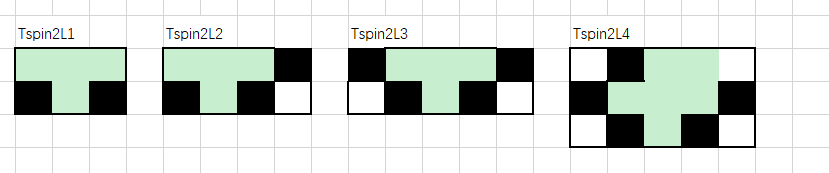
\includegraphics[width=1\textwidth]{figure/tSpinStruct.png}
    \captionof{figure}{T-spin结构图。绿色方块表示必须为空的位置,黑色表示必须有方块的位置,白色表示既可以有方块也可以为空的位置。}
\end{Figure}

\subsection{高阶评估函数}

传统俄罗斯方块AI在分析feature的时候可以对每个feature进行简单的线性判断,而基于现代规则的俄罗斯方块AI则不行。例如,将生存作为第一目标的传统俄罗斯方块AI会希望列高度越低越好,因为列高度越低生存的机会越大;而基于现代规则的俄罗斯方块AI则可能会希望列高度保持在4行左右,因为一次性消除4行所能对对方造成的攻击效果值得基于现代规则的俄罗斯方块AI冒这个险;除此之外,传统俄罗斯方块的AI往往会注重场地的平整,而搭建T-Spin则需要破坏这种平整,给T块空出一个凹槽。\\

这些就需要我们的AI采用和传统AI不同的对feature的evaluation方式。最终,我们决定使用多项式方式,给各个feature加上了他们的平方、三次方和四次方,得到了比之前更好的结果。

\section{训练结果评估}

在算法实现后,我们用1阶评估函数和4阶评估函数分别从零开始训练了1000个方块,同时记录每种函数在第一局游戏后,第50个方块后,第200个方块后,第1000个方块后的权重。为了评估这些训练结果,我们仿照真实对战环境建立了垃圾块模拟的功能。在AI游戏时,程序会在每个新方块生成时以不同概率随机生成不同行数的垃圾块,将场地内现有的方块往上顶。我们在垃圾块环境下对每个训练结果测试了五次(暂时关闭学习算法的更新),对相关统计数据取平均值进行分析以对AI的能力获得一个较全面的认识。每一局的统计数据包括死亡前消除的行数、得分的效率(总得分/处理的方块数)、多层消除的比率(2~4消)、连击的数量以及最终得分等。
\end{multicols}
\begin{table}[h]
    \centering
    \caption{使用一阶评估函数在训练了不同次数后的五次垃圾行环境测试中的平均指标}
    \begin{tabular}{@{}llllllllllll@{}}
    \toprule
          & 得分   & 方块    & 消行    & 单消率     & 二消率     & 三消率    & 四消率    & 二连率     & 三连率    & 四连率    & 五以上    \\ \midrule
    1局    & 434  & 91    & 30.2  & 80.80\% & 17.60\% & 1.60\% & 0.00\% & 12.80\% & 8.80\% & 0.00\% & 0.80\% \\
    50次   & 554  & 103.8 & 36.8  & 96.63\% & 3.37\%  & 0.00\% & 0.00\% & 12.92\% & 4.49\% & 2.25\% & 0.56\% \\
    200次  & 1392 & 217.2 & 92.4  & 79.78\% & 15.57\% & 3.28\% & 1.37\% & 15.57\% & 4.92\% & 0.00\% & 1.09\% \\
    1000次 & 3008 & 440.6 & 207.8 & 79.08\% & 16.30\% & 3.77\% & 0.85\% & 14.60\% & 5.96\% & 1.22\% & 0.49\% \\ \bottomrule
    \end{tabular}
\end{table}

\begin{table}[h]
    \centering
    \caption{使用四阶评估函数在训练了不同次数后的五次垃圾行环境测试中的平均指标}
    \begin{tabular}{@{}llllllllllll@{}}
    \toprule
          & 得分   & 方块    & 消行    & 单消率     & 二消率     & 三消率    & 四消率    & 二连率     & 三连率    & 四连率    & 五以上    \\ \midrule
    1局    & 888  & 140.6 & 55.8  & 92.25\% & 7.36\%  & 0.39\% & 0.00\% & 11.63\% & 6.20\% & 1.94\% & 1.16\% \\
    50块   & 1122 & 165   & 70    & 73.66\% & 20.99\% & 3.44\% & 1.91\% & 6.11\%  & 4.20\% & 2.29\% & 1.91\% \\
    200块  & 1848 & 255.4 & 117.6 & 67.88\% & 24.09\% & 5.11\% & 2.92\% & 11.68\% & 3.41\% & 0.73\% & 1.70\% \\
    1000块 & 3704 & 509.8 & 245.6 & 66.27\% & 24.97\% & 5.92\% & 2.84\% & 13.96\% & 6.15\% & 1.66\% & 0.71\% \\ \bottomrule
    \end{tabular}
    \end{table}

\begin{multicols}{2}

根据以上两张表格,我们能注意到在同样次数的训练中,使用4阶评估函数的训练的AI,在同样的垃圾行测试环境下,能够维持更长的时间,消去更多的行数,获取更高的分数。同时,随着训练次数的提升,无论是1阶AI还是4阶AI都获得了更好的表现,这与算法预期效果一致。另外,我们将多层消除率、连击比率、和单位方块得分均进行了画图比较。可以注意到在训练的过程中,AI开始慢慢学会这些获取高分的方法,多层消除和连击率都在逐步提高。尽管在第一局到第50块之间的学习效果不稳定,往后这些比率随着训练次数的提升均在逐渐提高。其中,一阶AI在学习连击方面更加迅速,但在1000块的长时间训练下与四阶AI的表现无太大差异,在多层消除方面(指一次操作同时消去多行),可以看到四阶AI的表现明显优于一阶AI。对应地,四阶AI在得分效率方面也优于1阶AI。

\end{multicols}

\begin{Figure}
    \centering
    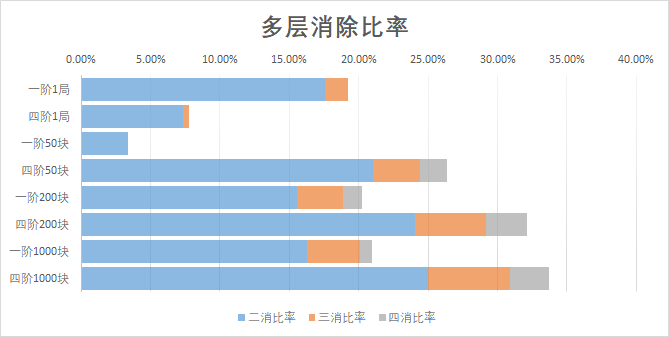
\includegraphics[width=0.7\textwidth]{figure/result1.png}
\end{Figure}

\begin{Figure}
    \centering
    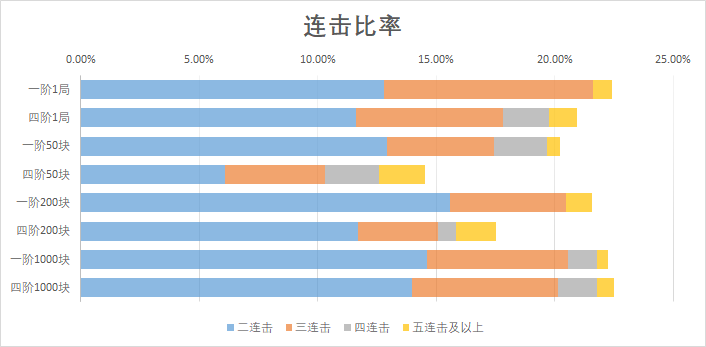
\includegraphics[width=0.7\textwidth]{figure/result2.png}
\end{Figure}

\begin{Figure}
    \centering
    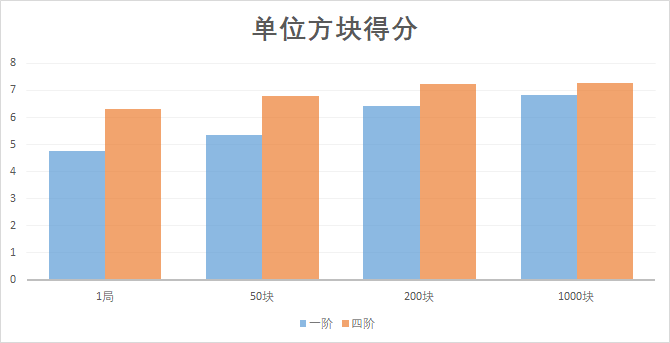
\includegraphics[width=0.7\textwidth]{figure/result3.png}
\end{Figure}


\begin{multicols}{2}

另外,在测试阶段,我们注意到没有一个AI在有意识地使用T-Spin操作获得高分,这可能是由于我们的评估函数中,仅有一个当前状态的T-Spin结构数量的Feature来鼓励AI使用T-Spin消除。而在真实的游戏环境中,绝大多数的T-spin消除都需要有意识地提前Hold一些T形方块,然后去构筑一些复杂的可以引起T-Spin的结构才能达成T-Spin消除。\\
而我们的方法仅在评估函数测算了T-Spin结构而没有进行搜索帮助完成T-Spin消除,因此,即使AI根据这个Feature能够感受到T-Spin的结构,但是由于做出T-Spin消除的条件较为苛刻,它难以将这个T-Spin结构顺利化为额外的加分。所以并没能很好地训练该权重。我们估计,在加入搜索和有关T-Spin的更多Feature后可以较好地达到主动去做T-Spin的目标。

\section{总结}

由于我们选择了一个基于pygame包开发的俄罗斯方块游戏,我们很大程度上依赖于这个游戏的初始设计。并且为了模拟对战,我们人为地修改了规则,特别是一些特殊操作的得分以鼓励AI主动去进行这些操作。但是实际上这些操作的得分在各个游戏中是不一样的。可能我们的模型并不能在其他俄罗斯方块的游戏中击败多数人类玩家。\\

另一方面,受限于Approximate Q-learnning的方法,我们只能寻找当前下落方块和已经hold的方块的leagal action。AI在游戏时可能会主动搭建诸如T-spin等特殊操作所需要的结构,但是并不能在对应的方块到来时使用。也就是说,我们的AI并不懂得在游戏中“运营”。 \\

在Action Search和矩阵匹配阶段,我们的算法设计相对简单,并不高效。这是因为我们使用了python进行开发,并不能很好地利用一些底层的优化来加速运算。\\

在训练中,我们的游戏和AI是同一线程,只有在完成Action Search并且找到最佳Action之后,AI才会移动方块到确定的地点。在真实的对战中,方块是自动下落的,并不会等待AI决定最佳Action。\\

如果可能,我们会将AI从pygame中解放出来,使用更加高效的工具重构为Double Q-learning或者Deep Q-learning的方法学习游戏的AI,并尝试在线上对战平台与真实人类玩家进行对战。\cite{ref1}

\end{multicols}

\section*{参考文献}

\begin{enumerate}[label={[\arabic*]}]
    \item Christophe Thiery, Bruno Scherrer, Christophe Thiery, Bruno Scherrer. Improvements on Learning Tetris with Cross Entropy. International Computer Games Association Journal, ICGA, 2009, 32. ffinria-00418930f
    \item Matt Stevens, Sabeek Pradhan. Playing Tetris with Deep Reinforcement Learning
    \item Ryan Heise. Playing TETRIS using the PageRank Algorithm. \url{https://www.ryanheise.com/tetris/tetris_artificial_intelligence.html}
    \item Misakamm, 传统规则俄罗斯方块AI技术介绍. \url{http://misakamm.com/blog/482}
\end{enumerate}


\end{document}